\subsection{Source of Demonstration}
\label{sec:source_of_demonstration}
Regarding the way how the expert demonstrations can be obtained, according to \cite{fang2019survey}, two categories can be identified: \begin{enumerate*}[label=\textbf{(\alph*)}]
    \item direct demonstration; 
    \item indirect demonstration.
\end{enumerate*}
\begin{figure}[htb]
     \centering
     \begin{subfigure}[b]{0.45\textwidth}
         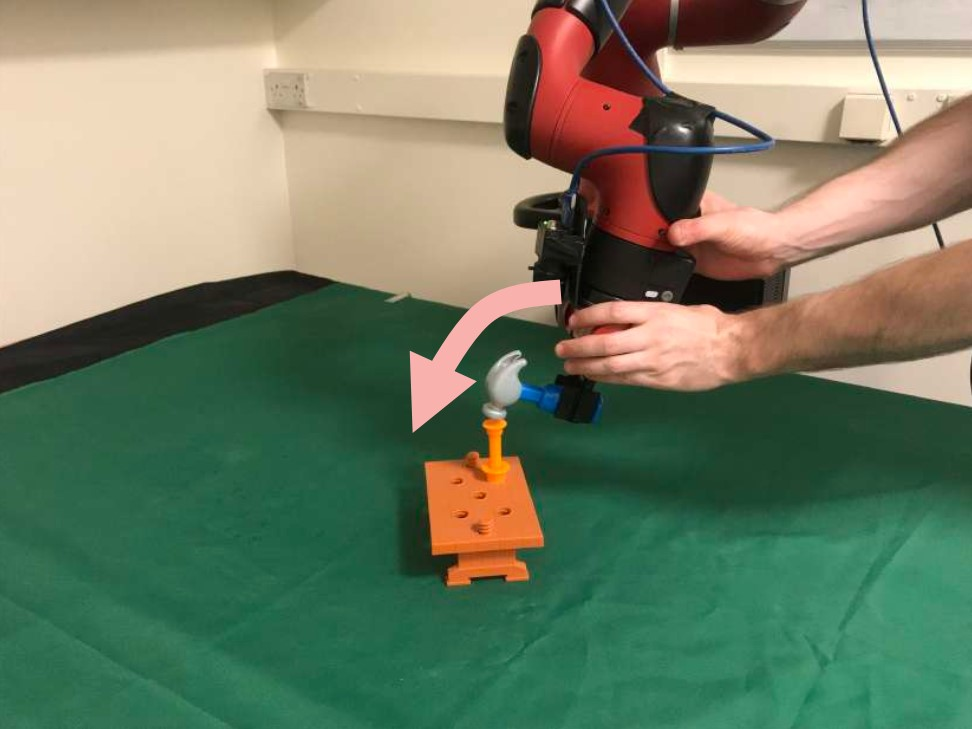
\includegraphics[width=\textwidth]{Figures/images/direct_demonstration/kinesthetic.jpg}
         \caption{Example of kinesthetic teaching \cite{johns2021coarse_to_fine}}
         \label{fig:kinesthetic}
     \end{subfigure}
     \hfill
     \begin{subfigure}[b]{0.5\textwidth}
         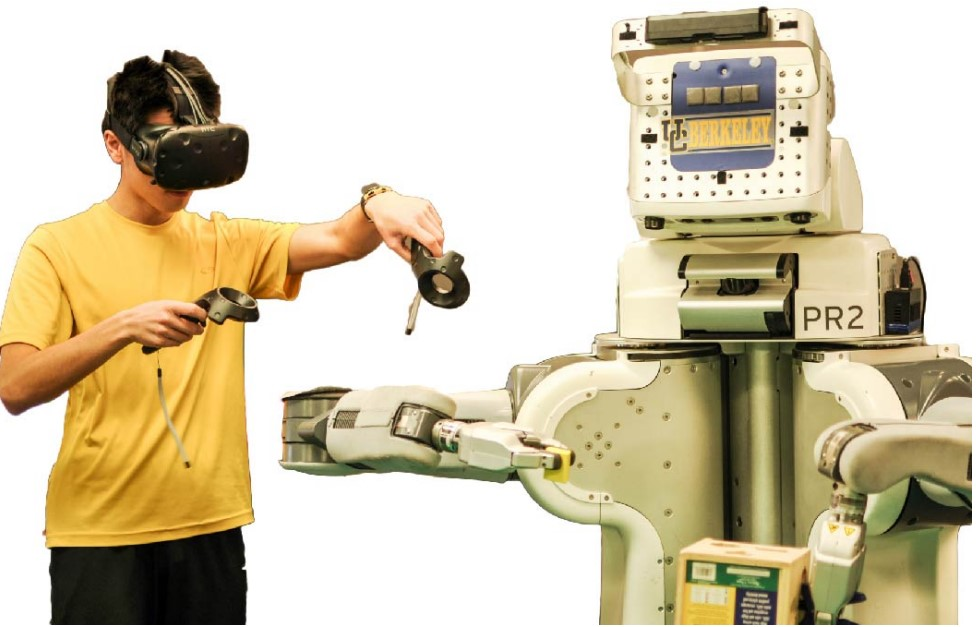
\includegraphics[width=\textwidth]{Figures/images/direct_demonstration/teleoperation.jpg}
         \caption{Example of teleoperation \cite{zhang2018deep_vr_teleoperation}}
         \label{fig:teleoperation}
     \end{subfigure}
    \hfill
    \caption{Examples of Direct Demonstration}
    \label{fig:direct_demonstrations}
\end{figure}


\paragraph{Direct Demonstration}  \mbox{} \\
\noindent It allows samples to be directly obtained from the robot, either with kinesthetic teaching (Figure \ref{fig:kinesthetic}) or teleoperation teaching (Figure \ref{fig:teleoperation}). In kinesthetic teaching the human operator contacts and guides the robot, that collects data by itself, while in teleoperation teaching the human operator remotely guides the robot with joystick, control panel, and wearable device. 
The former is characterized by the fact that there is no need to consider difference in kinematic between human and robot, as consequence, data has less noise. However, the robot must be passively controllable and require direct contact, introducing safety problems, and unintuitive demonstrations for robot with multiple degrees of freedom.
The latter is characterized by a higher safety, since there is no direct contact, and a wide application range.
A very popular example of teleoperation system is \textit{Roboturk} \cite{mandlekar2018roboturk}. It is a cloud-based teleoperation framework that enables the collection of high-scale demonstration dataset \cite{mandlekar2019scaling,mandlekar2022matters}, for both simulated and real-world robots, using a mobile-phone as controller (Figure \ref{fig:roboturk}). While this framework is interesting since it allows to collect data from a wide range of demonstrator with different demonstrations quality, it lacks of tactile information. When data are collected employing teleoperation, a way to collect contact information between the robot and the environment is represented by haptic interfaces \cite{cyberglove,touch}, which would allow the human operator to receive a force-feedback during teleoperation. However, the current literature has not yet focused on exploiting haptic information in the context of Learning from Demonstration, mainly due to the presence of open-challenges related to exploiting and best representing robot motion-related information, as will be explained in the following sections.
 \begin{figure}[htbp]
         \centering
         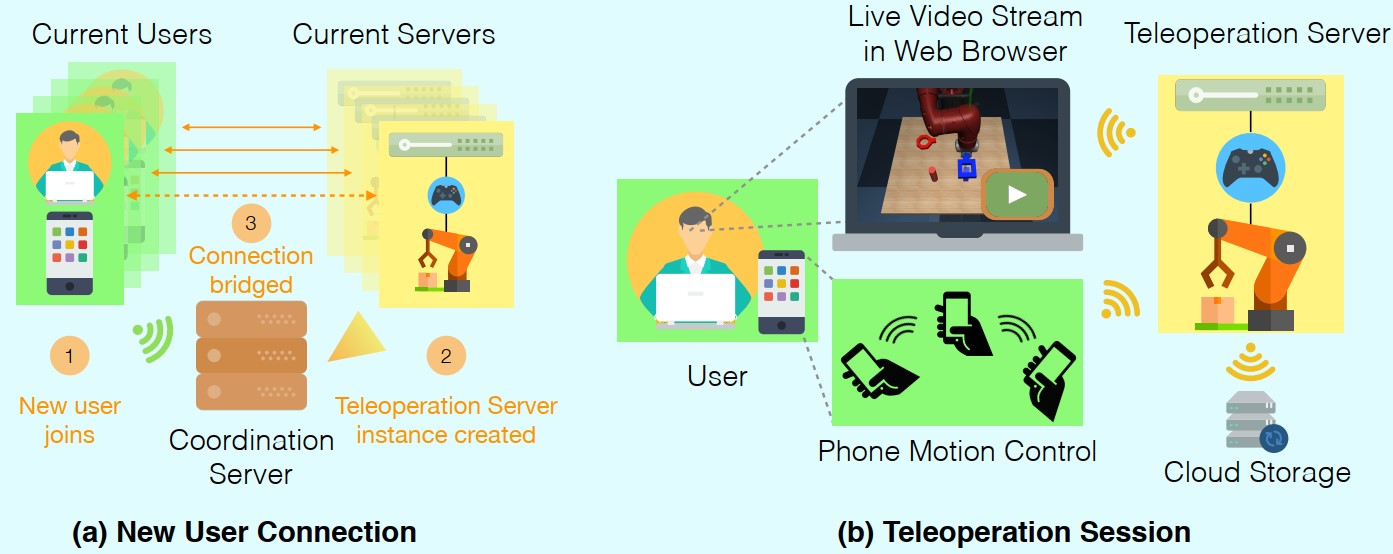
\includegraphics[width=0.8\textwidth]{Figures/images/indirect_demonstration/roboturk.jpg}
         \caption{System diagram of Roboturk \cite{mandlekar2018roboturk}}
         \label{fig:roboturk}
\end{figure}


\paragraph{Indirect Demonstration}  \mbox{} \\ 
It allows samples to be acquired in a way that is completely disconnected from the robot platform. In this case the human motion is recorded by vision system \cite{smith2019avid,sermanet2018time_contrastive} or wearable device \cite{liu2019_mirroring_without_overimitation}. In last years, the ability to extrapolate a policy starting from video of human performing a task has become a very important topic in the current literature \cite{fang2019survey,torabi2019recent_advances_lfo}. While Indirect Demonstration based on visual system allows to collect samples in the most intuitive and scalable way possible (potentially any video of performed task can be used), it lacks of tactile information, which can be obtained by using wearable devices such as gloves endowed with sensors able to measure the contact forces \cite{liu2017glove_force}. However, the correspondence problem must be solved, i.e., the system must be able to map motion captured in human space into the corresponding motion of the robot. In Section \ref{sec:lfo}, the different ways this problem has been solved in the context of visual demonstration will be explained in detail.
